\documentclass[UTF8]{ctexart}

\usepackage{ctex}
\CTEXsetup[format={\Large\bfseries}]{section}
\usepackage[top=28mm,bottom=28mm,left=15mm,right=15mm]{geometry}

\usepackage{fancyhdr}
\fancypagestyle{plain}{\pagestyle{fancy}}
\pagestyle{fancy}
\lhead{\kaishu 清华大学药学院药理毒理实验}
\newcommand{\numOfReport}[1]{\rhead{\kaishu 实验报告#1}}

\usepackage{fontspec}
\usepackage{wasysym}
\setCJKmainfont[AutoFakeBold={2}]{STZhongsong}
\setCJKmonofont{STZhongsong}

\usepackage{float}
\usepackage{booktabs}
\usepackage{tabularx}
\usepackage{array}
\usepackage{amsmath}
\usepackage{amsfonts}
\usepackage{amssymb}
\usepackage[figuresleft]{rotating}
\usepackage[para]{threeparttable}
\newcommand\info[2][40mm]{\underline{\makebox[#1][c]{#2}}}
\newcommand{\infoTable}[7]{
    \renewcommand\arraystretch{1.4}
    \begin{table}
        \begin{tabularx}{\textwidth}{
        >{\hsize=0.6\hsize\linewidth=\hsize}X
        >{\hsize=0.6\hsize\linewidth=\hsize}X
        >{\hsize=2.0\hsize\linewidth=\hsize}X
        >{\hsize=0.8\hsize\linewidth=\hsize}X
        }
            天气:\info[14mm]{#1} & 温度:\info[14mm]{#2 $^{\circ}\text{C}$} & 湿度:\info[14mm]{#3 $\%$} & 日期:#4\\
            姓名:\info[14mm]{#5} & 班级:\info[14mm]{#6} & 同组人:\info[70mm]{#7} & 
        \end{tabularx}
    \end{table}
}
\newcommand\columnC{\centering\arraybackslash}
\newcommand\columnL{\raggedright\arraybackslash}
\newcommand\columnR{\raggedleft\arraybackslash}

\usepackage{svg}
\usepackage{pdfpages}
\title{阿托品对乙酰胆碱的竞争性拮抗作用和 $\text{pA}_2$ 的测定}
\author{}
\numOfReport{五}

\begin{document}
\infoTable{晴}{13}{70}{10/23/2024}{何昱晖}{药3}{荣子健、马逸然、赵方一澜}
\date{}
\maketitle

\section{实验的目的和原理}

\subsection{实验目的}

\begin{itemize}
    \item [(1)] 观察阿托品对乙酰胆碱的竞争性拮抗作用;
    \item [(2)] 学习受体激动剂的量效关系曲线的绘制方法;
    \item [(3)] 掌握受体激动剂 $\text{pD}_2$ 和受体拮抗剂 $\text{pA}_2$ 的测定的方法和意义
\end{itemize}

\subsection{实验原理}

$\text{pD}_2$ 是评价受体激动剂的效应强度的指标,其定义为:能引起最大效应的 $50\%$ 时的药物剂量的\textbf{摩尔浓度负对数}。$\text{pD}_2=-\lg K_d$(其中 $K_d$ 是药物的解离常数)。其计算方法为:以 $E_x/E_{\max}$ 为纵坐标(其中 $E_x$ 是药物效应,$E_{\max}$ 是药物的最大效应,$\lg C$ 为横坐标作图,得到 S 型曲线,其中间部分为一条直线,计算纵坐标为 $0.5$ 时的横坐标值为 $\lg C_0$,取负数为 $\text{pD}_2$。

$\text{pA}_2$ 是一种用于来表示竞争性拮抗作用的强度指标,其意义是能使激动剂浓度提高到原来 2 倍时,可产生与原来浓度相同效应所需的拮抗剂浓度的负对数,$\text{pA}_2$ 值越大,说明拮抗剂的作用越强。其计算方法为:加入某定量的抑制剂后,再加入上述剂量的激动剂,以 $E_x/E_{\max}$ 为纵坐标,$\lg C$ 为横坐标作图,得到一条拟合直线,纵坐标为 $0.5$ 时,计算得到的横坐标值为 $\lg C_1$。

$$
    \text{pA}_2=\text{pA}_x+\lg\left(\frac{C_1}{C_0}-1\right)
$$

其中:

\begin{itemize}
    \item $\text{pA}_x$ 为拮抗剂摩尔浓度的负对数;
    \item $C_1$ 为加入拮抗剂后引起 $50\%$ 效应的激动剂摩尔浓度;
    \item $C_0$ 为引起 $50\%$ 效应的激动剂摩尔浓度。
\end{itemize}

公式推导过程:

根据占领模型,即激动剂占领受体的比例即为药效与最大药效的比例:

$$
    \frac{[\text{DR}]}{\text{R}_0}=\frac{[\text{D}]}{[\text{D}]+K_d}\Rightarrow C_0=K_d
$$

加入阿托品后可以计算 $C_1$:

$$
    \frac{[\text{DR}]}{[\text{R}_0]}=\dfrac{[\text{D}]}{\text{D}+K_d\left(1+\dfrac{[\text{A}_x]}{K_a}\right)}=\frac{1}{2}\Rightarrow\dfrac{C_1}{C_1+C_0\left(1+\dfrac{[\text{A}_x]}{K_a}\right)}=\frac{1}{2}\Rightarrow\frac{[\text{A}_x]}{K_a}=\frac{C_1}{C_0}-1
$$

又 $\text{pA}_2$ 定义为当激动剂浓度提高到原来的 2 倍时,可产生与原来浓度相同效应所需的拮抗剂浓度的负对数,得:

$$
    \frac{[\text{DR}]}{[\text{R}_0]}=\dfrac{2K_d}{2K_d+K_d\left(1+\dfrac{[\text{A}_2]}{K_a}\right)}=\frac{1}{2}\Rightarrow [\text{A}_2]=K_a
$$

因此

$$
    \frac{[\text{A}_x]}{[\text{A}_2]}=\frac{C_1}{C_0}-1\Rightarrow\text{pA}_2=\text{pA}_x+\lg\left(\frac{C_1}{C_0}-1\right)
$$

\section{实验材料}

\begin{itemize}
    \item 实验动物:豚鼠 1 只,$350\sim 500\text{g}$;
    \item 药品和试剂:阿托品($1\times10^{-7}\text{mol}/\text{L}$)、乙酰胆碱($10^{-2}$、$10^{-3}$、$10^{-4}$、$10^{-5}$、$10^{-6}$、$10^{-7}\text{mol}/\text{L}$)、台氏液、氧气等;
    \item 实验器材:离体组织灌流装置、麦氏浴槽、张力换能器、PowerLab 数据采集系统、注射器、外科手术器械等。
\end{itemize}

\section{实验方法}

\subsection{实验流程}

\begin{itemize}
    \item [1] PowerLab 仪器参数设置:使用「张力测定实验.adiset」文件,测试仪器使用 1 通道,设置参数采样速率为 $200/\text{s}$,量程 $10\text{g}$,调零;
    \item [2] 台氏液每组 $300\text{mL}$,$37^\circ\text{C}$ 保温,取 $20\text{mL}$ 用氧气饱和备用;
    \item [3] 麦氏浴槽中加 $20\text{mL}$ 台氏液,调节温度 $37\pm1^\circ\text{C}$,氧气 $2\sim 3$ 个气泡/秒;
    \item [4] 豚鼠回肠标本制备:取豚鼠,用木棒猛击头部处死,迅速解剖腹腔,找到回肠,剪取 20cm 左右回肠置于氧饱和台氏液中,剥离脂肪,用眼科剪剪成 $2\sim 2.5\text{cm}$ 左右的肠段,冲洗干净内容物。将肠管标本两端用缝针穿线,打结固定;一端打空结(约 $1\text{cm}$ 左右),另一端穿长线打结,用眼科镊钳住空结固定于弯钩上,放入麦氏浴槽,固定弯钩;将另一端长线与张力换能器相连;
    \item [5] 调整张力换能器高度,使得前负荷为 $5\sim 7\text{g}$ 左右;回肠标本在浴槽内平衡,每 10min 换液一次,共换液 3 次;
    \item [6] 最后一次换液后,浴槽中加入台氏液 20mL 平衡 10min,秒级一段正常曲线,随后按照表 1 次序,小剂量连续加入乙酰胆碱(Ach),制作 Ach 的累积效应曲线。每加一次药时都需标记,指标加药序号即可,直至曲线上升至最高峰不再升高为止。每次加样前,用移液枪先取出槽内相应体积的溶液,再加入药液;
    \item [7] 放掉麦氏浴槽中的溶液,用新鲜台氏液冲洗肠管 3 次,每次平衡 10 min,稳定标本共 30min,随后加入阿托品 0.2 mL(终浓度为 $10^{-9}\text{mol}/\text{L}$),1min 后加入乙酰胆碱,按照上述方法制作 Ach 累积效应曲线;
    \item [8] 实验结束,清洗所用容器和麦氏浴槽,关闭仪器。
\end{itemize}

\begin{table}[H]
    \centering
    \begin{threeparttable}[b]
        \caption{乙酰胆碱加样浓度和加样量}
        \quad

        \begin{tabularx}{\textwidth}{
            >{\columnC\hsize=0.6\hsize\linewidth=\hsize}X
            >{\columnC\hsize=1\hsize\linewidth=\hsize}X
            >{\columnC\hsize=1\hsize\linewidth=\hsize}X
            >{\columnC\hsize=1.4\hsize\linewidth=\hsize}X
        }
            \toprule[1.5pt]
            加药次序 & Ach 浓度($\text{mol}/\text{L}$) & 加入量(mL) & 浴槽中 Ach 累计浓度($\mu\text{mol}/\text{L}$)\\
            1 & $10^{-7}$ & 0.2 & 0.001\\
            2 & $10^{-7}$ & 0.4 & 0.003\\
            3 & $10^{-6}$ & 0.14 & 0.01\\
            4 & $10^{-6}$ & 0.4 & 0.03\\
            5 & $10^{-5}$ & 0.14 & 0.1\\
            6 & $10^{-5}$ & 0.4 & 0.3\\
            7 & $10^{-4}$ & 0.14 & 1\\
            8 & $10^{-4}$ & 0.4 & 3\\
            9 & $10^{-3}$ & 0.14 & 10\\
            10 & $10^{-3}$ & 0.4 & 30\\
            11 & $10^{-2}$ & 0.14 & 100\\
            12 & $10^{-2}$ & 0.4 & 300\\
            \bottomrule[1.5pt]
        \end{tabularx}
    \end{threeparttable}
\end{table}

\subsection{注意事项}

\begin{itemize}
    \item [1] 处死豚鼠取肠要迅速、轻巧,并置于氧饱和台氏液中保持活性;
    \item [2] 给予回肠肠管的前负荷不能太大(最开始时为 $5\sim 7\text{g}$,随着孵育时间的延长,其张力会降低);
    \item [3] 每次给予 Ach 时需等到前一次反应达到最大值时才能给下一个剂量的药物,即描记曲线到达平台阶段。制作整个累积量效曲线过程中不能换溶液;
    \item [4] 切勿随意更改生物信号处理采集系统的实验参数设置。
\end{itemize}

\section{实验结果}

图1是未加阿托品时测定的乙酰胆碱累积效应曲线图,平衡时的负荷约为 $4.5\text{g}$,最高值约为 $7\text{g}$:

\begin{figure}[H]
    \centering
    \includegraphics[width=12.5cm]{image-1.png}
    \caption{未加阿托品时的乙酰胆碱累积效应曲线}
\end{figure}

图2是加入阿托品时测定的乙酰胆碱累积效应曲线图,平衡时的负荷约为 $5.25\text{g}$,最高值约为 $7\text{g}$:

\begin{figure}[H]
    \centering
    \includegraphics[width=12.5cm]{image-2.png}
    \caption{加入阿托品时的乙酰胆碱累积效应曲线}
\end{figure}

表2是测定曲线中各段的平均值对比:

\begin{table}[H]
    \centering
    \begin{threeparttable}[b]
        \caption{对照组与实验组各阶段平均值比较}
        \quad

        \begin{tabularx}{\textwidth}{
            >{\columnC\hsize=1\hsize\linewidth=\hsize}X
            >{\columnC\hsize=1\hsize\linewidth=\hsize}X
            >{\columnC\hsize=1\hsize\linewidth=\hsize}X
        }
            \toprule[1.5pt]
            阶段 & 对照组 & 实验组 \\
            \midrule
            校准平衡 & 4.5377 & 5.2161\\
            加入阿托品 & / & 5.1461\\
            1 & 4.535 & 5.1459\\
            2 & 4.563 & 5.1417\\
            3 & 4.6307 & 5.1334\\
            4 & 4.9187 & 5.1393\\
            5 & 5.3415 & 5.2531\\
            6 & 5.8949 & 5.5183\\
            7 & 6.1906 & 6.0077\\
            8 & 6.4545 & 6.4767\\
            9 & 6.4946 & 6.6281\\
            10 & 6.5708 & 6.5234\\
            11 & 6.7552 & 6.5532\\
            12 & 6.7491 & 6.8002\\
            \bottomrule[1.5pt]
        \end{tabularx}
    \end{threeparttable}
\end{table}

对实验数据进行处理,对于对照组实验数据,可以发现加入编号 3 至 9 的数据拟合为一条直线时偏差较小,根据拟合结果可以得到:

$$
    \lg C_0=-\text{pD}_2=-6.6548
$$

对于实验组实验数据,可以发现加入编号 5 至 8 的数据拟合为一条直线时偏差较小,根据拟合结果可以得到:

$$
    \lg C_1=-6.0303
$$

因此可以得到最终的 $\text{pA}_2$ 为:

$$
    \begin{aligned}
        \text{pA}_2&=\text{pA}_x+\lg\left(\frac{C_1}{C_0}-1\right)\\
        &=-\lg(10^{-9})+\lg\left(\frac{10^{-6.0303}}{10^{-6.6548}}-1\right)\\
        &=9.5068
    \end{aligned}
$$

综上所述,阿托品的 $\text{pA}_2$ 为 9.5068,乙酰胆碱的 $\text{pD}_2$ 为 6.6548。

\begin{figure}[H]
    \centering
    \caption{实验数据处理}
    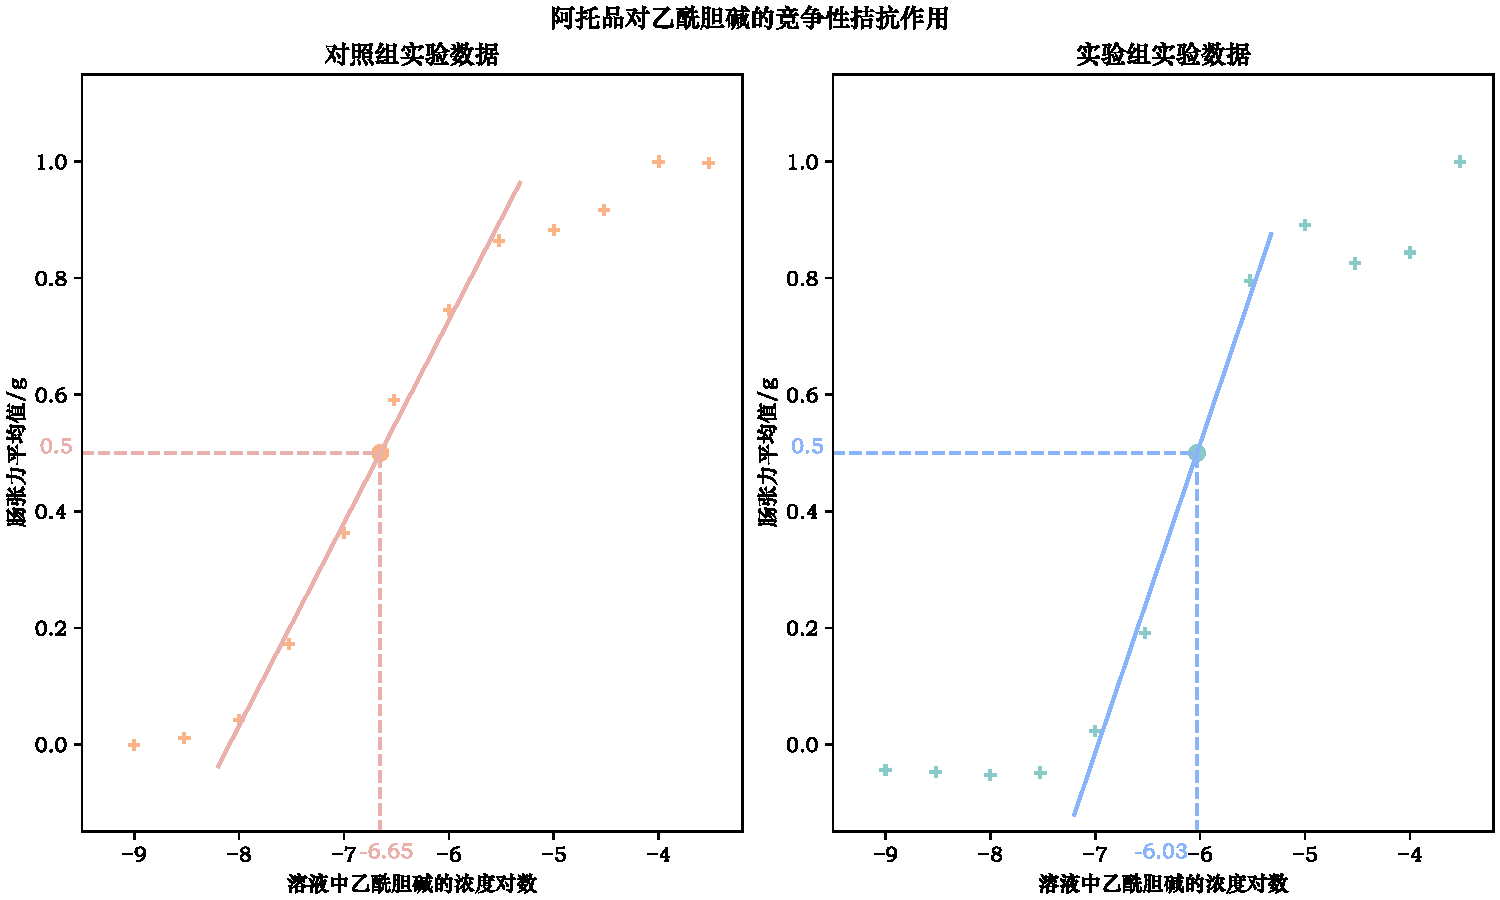
\includegraphics[scale=0.7]{figure-5_svg.pdf}
\end{figure}

\section{课后思考题}

\begin{itemize}
    \item [1] 请说明竞争性拮抗剂与非竞争性拮抗剂对激动剂的量效曲线的影响
    
        竞争性拮抗剂会使得激动剂的量效曲线的转折点延后,整体的效应也会减少;非竞争性拮抗剂会使得激动剂的量效曲线转折点延后,但是整体的效应不发生改变;
    
    \item [2] 请简述阿托品的药理作用
    
        阿托品可与乙酰胆碱竞争副交感神经节后纤维突触后膜的乙酰胆碱 M-受体,从而拮抗过量乙酰胆碱对突触后膜刺激所引起的毒蕈碱样症状和中枢神经症状;

    \item [3] 如果增加本实验中阿托品的用量,$\text{pA}_2$ 是否也会成比例增加?增加阿托品用量,乙酰胆碱量效曲线会如何变化?
    
        $\text{pA}_2$ 的值不会成比例增加。当增加阿托品用量时,乙酰胆碱的量效曲线的转折点会更加延后。

    \item [4] 为什么在实验中肠管收缩达到最大值后,会出现回肠收缩曲线反而下降的现象?
    
        因为肠管具有弹性,收缩至最远处后会回复。
\end{itemize}
\end{document}